% -----------------------------*- LaTeX -*------------------------------
\documentclass[UTF8]{article}
% ------------------------------------------------------------------------
% Packages
% ------------------------------------------------------------------------
\usepackage{ctex} % 支持中文
\usepackage[body={7in, 9in},left=1in,right=1in]{geometry} % 改变页边距
\usepackage{amsmath} % AMS 的数学宏包
\usepackage{amsfonts} % AMS 的数学字体宏包
\usepackage{amssymb} % AMS 符号库
\usepackage{bm} % 数学公式中的黑斜体
\usepackage{amsthm} % AMS 的定理环境宏包
\usepackage{graphicx} % 插图
\usepackage{subfigure} % 插子图
\usepackage{nicefrac} % 好看的分数
\usepackage{mathrsfs} % mathscr font
\usepackage{caption} % caption
\usepackage{algorithm,algorithmicx} % 伪代码支持宏包
\usepackage[noend]{algpseudocode} % 伪代码
\usepackage{fancyhdr} % 设置页眉、页脚
\usepackage{adjustbox} % 图片尺寸自动调整
\usepackage{esint} % 积分符号
\usepackage{mathtools} % 数学宏包的重要补充
\usepackage{upgreek} % 数学环境的直立希腊字母
\usepackage{enumitem} % 使用enumitem宏包, 改变列表项的格式
\usepackage{color} % 支持彩色
\usepackage{extarrows} % 任意长度的箭头
\usepackage{tikz} % 绘图
\usepackage{forest} % 绘树
\usepackage{xcolor} % 颜色宏包
\usepackage{breqn} % 公式自动换行
\usepackage{fontsize} % 字体大小
\usepackage[framemethod=TikZ]{mdframed} % 给文字加框
\usepackage{fontspec} % 字体库
\usepackage{bigstrut} % 用于表格中的换行
\usepackage{multirow} % 表格中多行单元格合并
\usepackage{multicol} % 表格中多列单元格合并
\usepackage{longtable} % 长表格
\usepackage{rotating} % 旋转图形和表格      以上三者用于绘制三线表
\usepackage{booktabs} % 三线表宏包
\usepackage{scribe} % Scribe 模板
\usepackage{diagbox} % 表格斜线
\usepackage{listings} % 插入代码
\usetikzlibrary{automata} % 引入automata库
\usetikzlibrary{shapes,arrows,positioning,chains} % 引入positioning库
% ------------------------------------------------------------------------
% Macros
% ------------------------------------------------------------------------
%~~~~~~~~~~~~~~~
% Utility latin
%~~~~~~~~~~~~~~~
\newcommand{\ie}{\textit{i.e.}}
\newcommand{\eg}{\textit{e.g.}}
%~~~~~~~~~~~~~~~
% Environment shortcuts
%~~~~~~~~~~~~~~~
\newcommand{\balign}[1]{\ealign{\begin{align}#1\end{align}}}
\newcommand{\baligns}[1]{\ealigns{\begin{align*}#1\end{align*}}}
\newcommand{\bitemize}[1]{\eitemize{\begin{itemize}#1\end{itemize}}}
\newcommand{\benumerate}[1]{\eenumerate{\begin{enumerate}#1\end{enumerate}}}
%~~~~~~~~~~~~~~~
% Text with quads around it
%~~~~~~~~~~~~~~~
\newcommand{\qtext}[1]{\quad\text{#1}\quad}
%~~~~~~~~~~~~~~~
% Shorthand for math formatting
%~~~~~~~~~~~~~~~
\newcommand{\mbb}[1]{\mathbb{#1}}
\newcommand{\mbi}[1]{\boldsymbol{#1}} % Bold and italic (math bold italic)
\newcommand{\mbf}[1]{\mathbf{#1}}
\newcommand{\mc}[1]{\mathcal{#1}}
\newcommand{\mrm}[1]{\mathrm{#1}}
\newcommand{\tbf}[1]{\textbf{#1}}
\newcommand{\tsc}[1]{\textsc{#1}}
%\def\\langle {{\langle }}
%\def\\rangle {{\rangle }}
\newcommand{\sT}{\sf T}
\newcommand{\grad}{\nabla}
\newcommand{\Proj}{\Pi}
%~~~~~~~~~~~~~~~
% Common sets 定义数集符号
%~~~~~~~~~~~~~~~
\newcommand{\R}{\mathbb{R}}
\newcommand{\Z}{\mathbb{Z}}
\newcommand{\Q}{\mathbb{Q}}
\newcommand{\N}{\mathbb{N}}
\newcommand{\C}{\mathbb{C}}
\newcommand{\reals}{\mathbb{R}} % Real number symbol
\newcommand{\integers}{\mathbb{Z}} % Integer symbol
\newcommand{\rationals}{\mathbb{Q}} % Rational numbers
\newcommand{\naturals}{\mathbb{N}} % Natural numbers
\newcommand{\complex}{\mathbb{C}} % Complex numbers
%~~~~~~~~~~~~~~~
% Common functions
%~~~~~~~~~~~~~~~
\renewcommand{\exp}[1]{\operatorname{exp}\left(#1\right)} % Exponential
\newcommand{\indic}[1]{\mbb{I}\left(#1\right)} % Indicator function
\newcommand{\indicsub}[2]{\mbb{I}_{#2}\left(#1\right)} % Indicator function
\newcommand{\argmax}{\mathop\mathrm{arg\, max}} % Defining math symbols
\newcommand{\argmin}{\mathop\mathrm{arg\, min}}
\renewcommand{\arccos}{\mathop\mathrm{arccos}}
\newcommand{\dom}{\mathop\mathrm{dom}} % Domain
\newcommand{\range}{\mathop\mathrm{range}} % Range
\newcommand{\diag}{\mathop\mathrm{diag}}
\newcommand{\tr}{\mathop\mathrm{tr}}
\newcommand{\abs}{\mathop\mathrm{abs}}
\newcommand{\card}{\mathop\mathrm{card}}
\newcommand{\sign}{\mathop\mathrm{sign}}
\newcommand{\prox}{\mathrm{prox}} % prox
\newcommand{\rank}[1]{\mathrm{rank}(#1)}
\newcommand{\supp}[1]{\mathrm{supp}(#1)}
\newcommand{\norm}[1]{\lVert#1\rVert}
%~~~~~~~~~~~~~~~
% Common probability symbols
%~~~~~~~~~~~~~~~
\newcommand{\family}{\mathcal{P}} % probability family / statistical model
\newcommand{\iid}{\stackrel{\mathrm{iid}}{\sim}}
\newcommand{\ind}{\stackrel{\mathrm{ind}}{\sim}}
\newcommand{\E}{\mathbb{E}} % Expectation symbol
\newcommand{\Earg}[1]{\E\left[#1\right]}
\newcommand{\Esubarg}[2]{\E_{#1}\left[#2\right]}
\renewcommand{\P}{\mathbb{P}} % Probability symbol
\newcommand{\Parg}[1]{\P\left(#1\right)}
\newcommand{\Psubarg}[2]{\P_{#1}\left[#2\right]}
%\newcommand{\Cov}{\mrm{Cov}} % Covariance symbol
%\newcommand{\Covarg}[1]{\Cov\left[#1\right]}
%\newcommand{\Covsubarg}[2]{\Cov_{#1}\left[#2\right]}
%\newcommand{\model}{\mathcal{P}} % probability family / statistical model
%~~~~~~~~~~~~~~~
% Distributions
%~~~~~~~~~~~~~~~
%\newcommand{\Gsn}{\mathcal{N}}
%\newcommand{\Ber}{\textnormal{Ber}}
%\newcommand{\Bin}{\textnormal{Bin}}
%\newcommand{\Unif}{\textnormal{Unif}}
%\newcommand{\Mult}{\textnormal{Mult}}
%\newcommand{\NegMult}{\textnormal{NegMult}}
%\newcommand{\Dir}{\textnormal{Dir}}
%\newcommand{\Bet}{\textnormal{Beta}}
%\newcommand{\Gam}{\textnormal{Gamma}}
%\newcommand{\Poi}{\textnormal{Poi}}
%\newcommand{\HypGeo}{\textnormal{HypGeo}}
%\newcommand{\GEM}{\textnormal{GEM}}
%\newcommand{\BP}{\textnormal{BP}}
%\newcommand{\DP}{\textnormal{DP}}
%\newcommand{\BeP}{\textnormal{BeP}}
%\newcommand{\Exp}{\textnormal{Exp}}
%~~~~~~~~~~~~~~~
% Theorem-like environments
%~~~~~~~~~~~~~~~
%\theoremstyle{definition}
%\newtheorem{definition}{Definition}
%\newtheorem{example}{Example}
%\newtheorem{problem}{Problem}
%\newtheorem{lemma}{Lemma}
%~~~~~~~~~~~~~~~
% 组合数学的模板和作业里用到的一些宏包和自定义命令
%~~~~~~~~~~~~~~~
\renewcommand{\emph}[1]{\begin{kaishu}#1\end{kaishu}}
\newcommand{\falfac}[1]{^{\underline{#1}}}
\newcommand{\binomfrac}[2]{\frac{#1^{\underline{#2}}}{#2!}}
\newcommand{\ceil}[1]{\left\lceil #1 \right\rceil}
\newcommand{\floor}[1]{\left\lfloor #1 \right\rfloor}
\newcommand{\suminfty}[2]{\sum_{#1=#2}^{\infty}}
\newcommand{\suminftyk}[0]{\sum_{k=0}^{\infty}}
\newcommand{\sumint}[3]{\sum_{#1=#2}^{#3}}
\newcommand{\sumintk}[2]{\sum_{k=#1}^{#2}}
\newcommand{\suminti}[2]{\sum_{i=#1}^{#2}}
%~~~~~~~~~~~~~~~
% 定义新命令
%~~~~~~~~~~~~~~~
\newcommand*{\unit}[1]{\mathop{}\!\mathrm{#1}}
\newcommand*{\dif}{\mathop{}\!\mathrm{d}}%微分算子 d
\newcommand*{\pdif}{\mathop{}\!\partial}%偏微分算子
\newcommand*{\cdif}{\mathop{}\!\nabla}%协变导数、nabla 算子
\newcommand*{\laplace}{\mathop{}\!\Delta}%laplace 算子
\newcommand*{\deri}[1]{\mathrm{d} #1}
\newcommand*{\deriv}[2]{\frac{\mathrm{d} #1}{\mathrm{d} {#2}}}
\newcommand*{\derivh}[3]{\frac{\mathrm{d}^{#1} #2}{\mathrm{d} {#3^{#1}}}}
\newcommand*{\pderiv}[2]{\frac{\partial #1}{\partial {#2}}}
\newcommand*{\pderivh}[3]{\frac{\partial^{#1} #2}{\partial {#3^{#1}}}}
\newcommand*{\dderiv}[2]{\dfrac{\mathrm{d} #1}{\mathrm{d} {#2}}}
\newcommand*{\dderivh}[3]{\dfrac{\mathrm{d}^{#1} #2}{\mathrm{d} {#3^{#1}}}}
\newcommand*{\dpderiv}[2]{\dfrac{\partial #1}{\partial {#2}}}
\newcommand*{\dpderivh}[3]{\dfrac{\partial^{#1} #2}{\partial {#3^{#1}}}}
\newcommand{\me}[1]{\mathrm{e}^{#1}}%e 指数
\newcommand{\mi}{\mathrm{i}}%虚数单位
%\newcommand{\mc}{\mathrm{c}}%光速 定义与mathcal冲突
\newcommand{\red}[1]{\textcolor{red}{#1}}
\newcommand{\blue}[1]{\textcolor{blue}{#1}}
%\newcommand{\Rome}[1]{\setcounter{rome}{#1}\Roman{rome}}
%~~~~~~~~~~~~~~~
% 公式环境中箭头符号的简写
%~~~~~~~~~~~~~~~
\newcommand{\ra}{\rightarrow}
\newcommand{\Ra}{\Rightarrow}
\newcommand{\la}{\leftarrow}
\newcommand{\La}{\Leftarrow}
\newcommand{\lra}{\leftrightarrow}
\newcommand{\Lra}{\Leftrightarrow}
\newcommand{\lgla}{\longleftarrow}
\newcommand{\Lgla}{\Longleftarrow}
\newcommand{\lgra}{\longrightarrow}
\newcommand{\Lgra}{\Longrightarrow}
\newcommand{\lglra}{\longleftrightarrow}
\newcommand{\Lglra}{\Longleftrightarrow}
%~~~~~~~~~~~~~~~
% 一些数学的环境设置
%~~~~~~~~~~~~~~~
%\newcounter{counter_exm}\setcounter{counter_exm}{1}
%\newcounter{counter_prb}\setcounter{counter_prb}{1}
%\newcounter{counter_thm}\setcounter{counter_thm}{1}
%\newcounter{counter_lma}\setcounter{counter_lma}{1}
%\newcounter{counter_dft}\setcounter{counter_dft}{1}
%\newcounter{counter_clm}\setcounter{counter_clm}{1}
%\newcounter{counter_cly}\setcounter{counter_cly}{1}
\newtheorem{theorem}{{\hskip 1.7em \bf 定理}}
\newtheorem{lemma}[theorem]{\hskip 1.7em 引理}
\newtheorem{proposition}[theorem]{\hskip 1.7em 命题}
\newtheorem{claim}[theorem]{\hskip 1.7em 断言}
\newtheorem{corollary}[theorem]{\hskip 1.7em 推论}
% \newcommand{\problem}[1]{{\setlength{\parskip}{10pt}\noindent \bf{#1}}}
\newenvironment{solution}{{\noindent \bf 解 \quad}}{}
\newenvironment{remark}{{\noindent \bf 注 \quad}}{}
\newenvironment{definition}{{\noindent \bf 定义 \quad}}{}
\renewenvironment{proof}{{\setlength{\parskip}{7pt}\noindent\hskip 2em \bf 证明 \quad}}{\hfill$\qed$\par}
\newenvironment{example}{{\noindent\bf 例 \quad}}{\hfill$\qed$\par}
%\newenvironment{concept}[1]{{\bf #1\quad} \begin{kaishu}} {\end{kaishu}\par}
%~~~~~~~~~~~~~~~
% 本.tex文档中特殊定义命令
%~~~~~~~~~~~~~~~
\newcommand{\lno}[1]{\overline{#1}}
\newcommand{\NP}{\mathrm{NP}}
\newcommand{\coNP}{\mathrm{coNP}}
% \newcommand{\ISO}{\mathrm{ISO}}
\newcommand{\SAT}{\mathrm{SAT}}
\newcommand{\USAT}{\mathrm{USAT}}
% \newcommand{\threeSAT}{\mathrm{3\text{-}SAT}}
\renewcommand{\P}{\mathrm{P}}
% \mathchardef\mhyphen="2D
% \newcommand{\CNF}{\mathrm{CNF}}
% \newcommand{\DNF}{\mathrm{DNF}}
% \newcommand{\SetSp}{\mathrm{SET\text{-}SPLITTING}}
% \newcommand{\PUZZLE}{\mathrm{PUZZLE}}
% \newcommand{\SPATH}{\mathrm{SPATH}}
% \newcommand{\LPATH}{\mathrm{LPATH}}
% \newcommand{\UHAMPATH}{\mathrm{UHAMPATH}}
\newcommand{\SPACE}{\mathrm{SPACE}}
\newcommand{\NSPACE}{\mathrm{NSPACE}}
\newcommand{\PSPACE}{\mathrm{PSPACE}}
\newcommand{\NPSPACE}{\mathrm{NPSPACE}}
\newcommand{\DFA}{\mathrm{DFA}}
\newcommand{\NFA}{\mathrm{NFA}}
\newcommand{\TQBF}{\mathrm{TQBF}}
% \newcommand{\L}{\mathrm{L}}
\renewcommand{\O}{\mathrm{O}}
\newcommand{\NL}{\mathrm{NL}}
\newcommand{\coNL}{\mathrm{coNL}}
\newcommand{\LADDER}{\mathrm{LADDER_{DFA}}}
\newcommand{\hd}{\mathrm{\text{-}hard}}
\newcommand{\ADD}{\mathrm{ADD}}
\newcommand{\STCN}{\mathrm{STRONGLY\text{-}CONNECTED}}
\newcommand{\PATH}{\mathrm{PATH}}
\newcommand{\A}{\mathrm{A}}
%使用align环境公式换页
\allowdisplaybreaks[4]

\definecolor{dkgreen}{rgb}{0,0.6,0}
\definecolor{gray}{rgb}{0.5,0.5,0.5}
\definecolor{mauve}{rgb}{0.58,0,0.82}
\lstset{
  frame=tb,
  aboveskip=3mm,
  belowskip=3mm,
  showstringspaces=false,
  columns=flexible,
  framerule=1pt,
  rulecolor=\color{gray!35},
  backgroundcolor=\color{gray!5},
  basicstyle={\small\ttfamily},
  numbers=none,
  numberstyle=\tiny\color{gray},
  keywordstyle=\color{blue},
  commentstyle=\color{dkgreen},
  stringstyle=\color{mauve},
  breaklines=true,
  breakatwhitespace=true,
  tabsize=3,
}

\setmainfont{Times New Roman}
\setsansfont{Times New Roman}
\setmonofont{Menlo}
\setCJKmainfont{STHeiti}
\setCJKsansfont{STSong}
\setCJKmonofont{STFangsong}
\punctstyle{kaiming}

\begin{document}

\pagestyle{fancy}
\lhead{\emph{操作系统}}
\chead{\emph{中国科学院大学}}
\rhead{\emph{2022K800992910张家玮}}

\begin{center}
    {\LARGE \bf 第三次作业}
\end{center}

\tbf{3.1}

\begin{enumerate}[label=(\arabic*)]
    \item 所写C程序如下:
    
    \begin{lstlisting}[language=C]
        #include <stdio.h>
        #include <time.h>
        #include <stdlib.h>
        #include <unistd.h>

        int main(){
            int array[1000000];
            for (int i = 0; i < 1000000; i++)
                array[i] = i;
            int sum = 0;
            struct timespec start, end;
            clock_gettime(CLOCK_MONOTONIC, &start);
            for (int i = 0; i < 1000000; i++)
                sum += array[i];
            clock_gettime(CLOCK_MONOTONIC, &end);
            printf("Sum: %d\n", sum);
            printf("Time: %ld ns\n", (end.tv_sec - start.tv_sec) * 1000000000 + (end.tv_nsec - start.tv_nsec));
            return 0;
        }
    \end{lstlisting}

    编译运行后,输出结果如下:

    \begin{figure}[H]
        \centering
        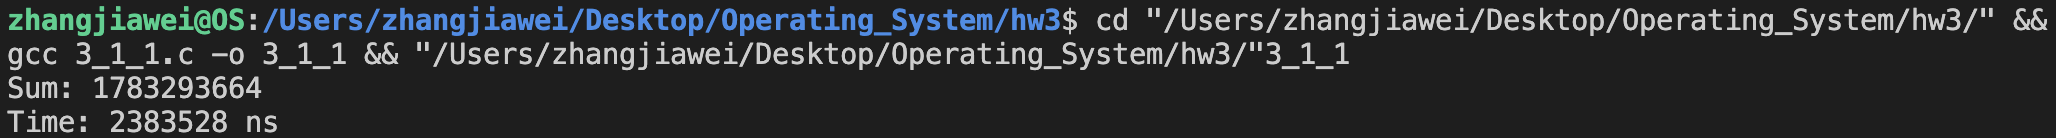
\includegraphics[width=\textwidth]{3_1_1.png}
        \caption{3_1_1运行结果}
    \end{figure}

    \item 所写C程序如下:
    
    \begin{lstlisting}[language=C]
        #include <stdio.h>
        #include <time.h>
        #include <stdlib.h>
        #include <unistd.h>
        #include <pthread.h>
        #define THREADS 4
        int sum[THREADS] = {0};
        int array[1000000];
        
        typedef struct {
            int *array;
            int id;
        } thread_data_t;
        
        void* thread_sum(void* arg){
            thread_data_t *data = (thread_data_t*)arg;
            int *array = data->array;
            int id = data->id;
            int local_sum = 0;
            int start = id * 1000000 / THREADS;
            int end = (id + 1) * 1000000 / THREADS;
            for (int i = start; i < end ; i++)
                local_sum += array[i];
            sum[id] = local_sum;
            return NULL;
        }
        
        int main(){    
            for (int i = 0; i < 1000000; i++)
                array[i] = i;
        
            struct timespec start, end;
            pthread_t threads[THREADS];
            thread_data_t thread_data[THREADS];
            clock_gettime(CLOCK_MONOTONIC, &start);
            for (int i = 0; i < THREADS; i++){
                thread_data[i].array = array;
                thread_data[i].id = i;
                pthread_create(&threads[i], NULL, thread_sum, &thread_data[i]);
            }
            for (int i = 0; i < THREADS; i++)
                pthread_join(threads[i], NULL);
        
            int total_sum = 0;
            for (int i = 0; i < THREADS; i++)
                total_sum += sum[i];
            clock_gettime(CLOCK_MONOTONIC, &end);
            printf("Sum: %d\n", total_sum);
            printf("Time: %ld ns\n", (end.tv_sec - start.tv_sec) * 1000000000 + (end.tv_nsec - start.tv_nsec));
            return 0;
        }
    \end{lstlisting}

    在这个程序中,我将数组分成了四份,分别由四个线程进行求和,最后将四个线程的结果相加得到最终结果。

    编译运行后,输出结果如下:

    \begin{figure}[H]
        \centering
        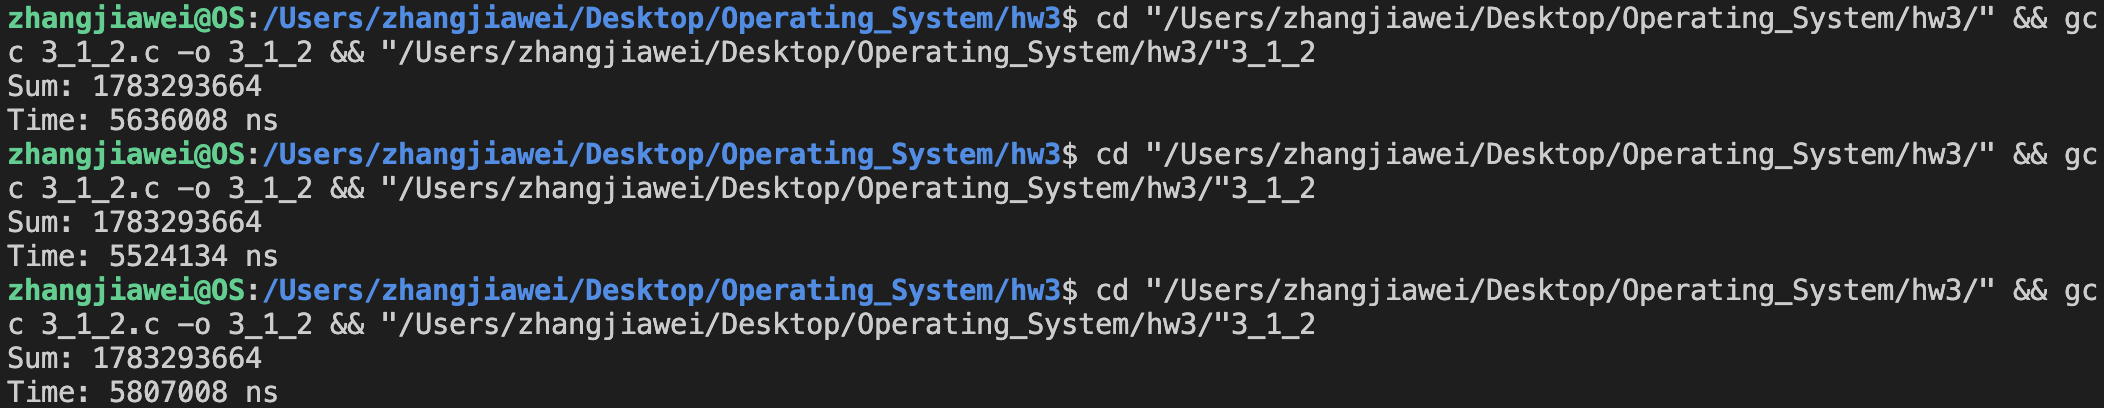
\includegraphics[width=\textwidth]{3_1_2.png}
        \caption{3_1_2运行结果}
    \end{figure}

    可以看出,四线程的运行时间大于直接进行求和的运行时间,这是因为线程的创建和销毁也需要时间,而且线程之间的切换也会带来额外的开销。经过进一步试验,发现随着线程数目从1开始逐渐增加,程序运行时间先降低后增加,这是因为我的CPU是8核的,当线程数目增加到8时,线程数目超过了CPU的核心数,导致线程切换的开销增加,从而使得程序运行时间增加。

    \item 所写C程序如下:
    
    \begin{lstlisting}[language=C]
        #define _GNU_SOURCE 
        // There may be some wrong with the homework document, if the macro is __USE_GNU, the program will not run. After asking Github copilot, I change it to _GNU_SOURCE, and the program runs successfully. I don't know if others have the same problem.
        #include <stdio.h>
        #include <time.h>
        #include <stdlib.h>
        #include <unistd.h>
        #include <pthread.h>
        #include <sched.h>
        #define THREADS 4
        int array[1000000];
        int sum[THREADS] = {0};
        
        typedef struct {
            int *array;
            int id;
        } thread_data_t;
        
        void* thread_sum(void* arg){
            thread_data_t *data = (thread_data_t*)arg;
            int *array = data->array;
            int id = data->id;
            int local_sum = 0;
            int start = id * 1000000 / THREADS;
            int end = (id + 1) * 1000000 / THREADS;
            for (int i = start; i < end; i++)
                local_sum += array[i];
            sum[id] = local_sum;
            return NULL;
        }
        
        void* worker(void* arg){
            thread_data_t *data = (thread_data_t*)arg;
            int core_id = data->id;
            cpu_set_t cpuset;
            CPU_ZERO(&cpuset);
            CPU_SET(core_id, &cpuset);
            sched_setaffinity(0, sizeof(cpuset), &cpuset);
            thread_sum(arg);
            return NULL;
        }
        
        int main(){    
            for (int i = 0; i < 1000000; i++)
                array[i] = i;
        
            struct timespec start, end;
            pthread_t threads[THREADS];
            thread_data_t thread_data[THREADS];
            clock_gettime(CLOCK_MONOTONIC, &start);
            for (int i = 0; i < THREADS; i++){
                thread_data[i].array = array;
                thread_data[i].id = i;
                pthread_create(&threads[i], NULL, worker, &thread_data[i]);
            }
            for (int i = 0; i < THREADS; i++)
                pthread_join(threads[i], NULL);
        
            int total_sum = 0;
            for (int i = 0; i < THREADS; i++)
                total_sum += sum[i];
            clock_gettime(CLOCK_MONOTONIC, &end);
            printf("Sum: %d\n", total_sum);
            printf("Time: %ld ns\n", (end.tv_sec - start.tv_sec) * 1000000000 + (end.tv_nsec - start.tv_nsec));
            return 0;
        }
    \end{lstlisting}

    在这个程序中,我将线程绑定到了特定的CPU核心上,这样可以避免线程切换的开销。编译运行后,输出结果如下:

    \begin{figure}[H]
        \centering
        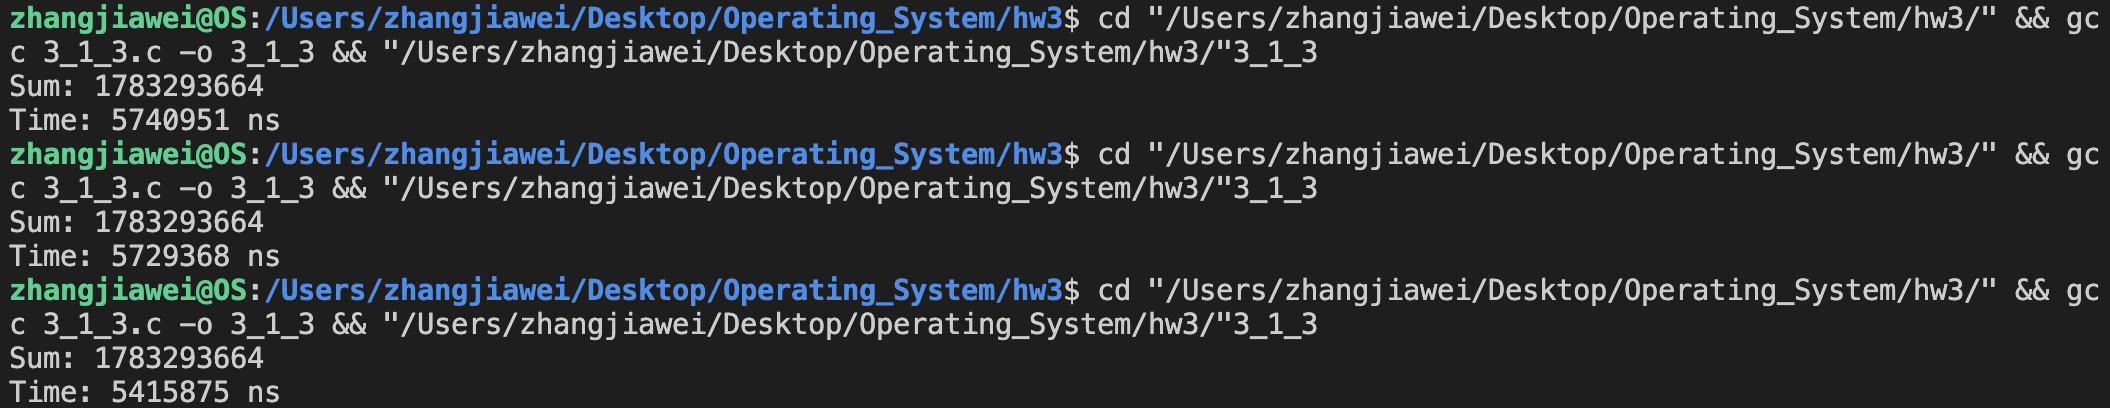
\includegraphics[width=\textwidth]{3_1_3.png}
        \caption{3_1_3运行结果}
    \end{figure}

    运行的结果与上一问相差无几,这可能是由于操作系统在上一问中自动进行了线程绑定,所以运行时间没有太大的变化。
\end{enumerate}

\tbf{3.2}

所写C程序如下:

\begin{lstlisting}[language=C]
    #include <stdio.h>
    #include <time.h>
    #include <stdlib.h>
    #include <unistd.h>
    #include <pthread.h>
    #define THREADS 4 // Number of threads
    int array[1000000];
    struct thread_data_t
    {
        int *array;
        int id;
    }; // Structure to pass data to threads
    
    // Function to assign values to array
    void* thread_assign(void* arg){
        struct thread_data_t *data = (struct thread_data_t*)arg; // Get data from argument
        int *array = data->array; // Get array from data
        int id = data->id; // Get id from data to calculate start and end index of current thread
        int start = id * 1000000 / THREADS; // Calculate start index
        int end = (id + 1) * 1000000 / THREADS; // Calculate end index
        for (int i = start; i < end; i++)
            array[i] = i;
        return NULL;
    }
    
    int main(){
        struct thread_data_t thread_data[THREADS]; // Array of thread data to pass to threads
        pthread_t threads[THREADS]; // Array of threads to store thread ids
        for (int i = 0; i < THREADS; i++){
            thread_data[i].array = array;
            thread_data[i].id = i;
            pthread_create(&threads[i], NULL, thread_assign, &thread_data[i]); // Create threads and pass data to them
        }
        for (int i = 0; i < THREADS; i++)
            pthread_join(threads[i], NULL); // Wait for threads to finish
    
        int sum = 0;
        for (int i = 0; i < 1000000; i++)
            sum += array[i];
        printf("Sum: %d\n", sum);
        return 0;
    }
\end{lstlisting}

在这个程序中,我将数组分成了四份,分别由四个线程进行赋值,最后将整个数组的值相加得到最终结果。编译运行后,输出结果如下:

\begin{figure}[H]
    \centering
    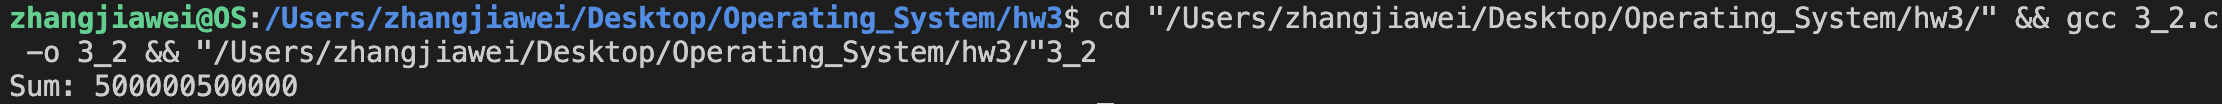
\includegraphics[width=\textwidth]{3_2.png}
    \caption{3_2运行结果}
\end{figure}
\end{document}